\documentclass[11pt]{article}
\usepackage{amssymb}
\usepackage[english]{babel}
\usepackage{fullpage}
\usepackage{graphicx}
\graphicspath{ {./images/} }
\usepackage{spverbatim}
\usepackage{listings}
\usepackage{color}
\usepackage{soul}

\definecolor{dkgreen}{rgb}{0,0.6,0}
\definecolor{gray}{rgb}{0.5,0.5,0.5}
\definecolor{mauve}{rgb}{0.58,0,0.82}

\lstset{frame=tb,
  language=Java,
  aboveskip=3mm,
  belowskip=3mm,
  showstringspaces=false,
  columns=flexible,
  basicstyle={\small\ttfamily},
  numbers=none,
  numberstyle=\tiny\color{gray},
  keywordstyle=\color{blue},
  commentstyle=\color{dkgreen},
  stringstyle=\color{mauve},
  breaklines=true,
  breakatwhitespace=true,
  tabsize=3
}

\def\titre{}
\def\auteur{}
\def\courriel{}



\makeatletter

\title{INF6306\\Patrons pour la compr\'{e}hension de programme}

\author{
    Foutse Khomh \\
    D\'{e}partement G\'{e}nie Informatique et G\'{e}nie Logiciel \\
    \'{E}cole Polytechnique de Montr\'{e}al, Qu\'{e}bec, Canada \\
    \texttt{foutse.khomh@polymtl.ca}
}

\date{}



\begin{document}
\maketitle

\section{Identification}

\paragraph{First, last name of the students:} Javier Rosales, Isabella Ferreira, Mahmood Vahedi\auteur 
\paragraph{Date:} November 16, 2018

\paragraph{Practice 1}\titre

\section{Abstract Factory}

The abstract factory pattern provides a way to encapsulate a group of individual factories that have a common theme without specifying their concrete classes. In normal usage, the client software creates a concrete implementation of the abstract factory and then uses the generic interface of the factory to create the concrete objects that are part of the theme. The client does not know which concrete objects it gets from each of these internal factories since it uses only the generic interfaces of their products. This pattern separates the details of implementation of a set of objects from their general usage and relies on object composition, as object creation is implemented in methods exposed in the factory interface.

\subsection*{Example}

Figure~\ref{fig:abstract_factory} presents the UML diagram of the Abstract Factory design pattern in the project \textit{openjms}. The abstract class \texttt{AbstractHTTPManagedConnectionFactory} plays the role of \textit{abstract factory}, and the class \texttt{HTTPManagedConnectionFactory} plays the role of \textit{concrete factory}. Additionally, \texttt{ConnectionFactory}, \texttt{Managed\\Connection}, and \texttt{ManagedConnectionAcceptor} play the role of \textit{products}.\\

\begin{figure}[htb]
    \centering
    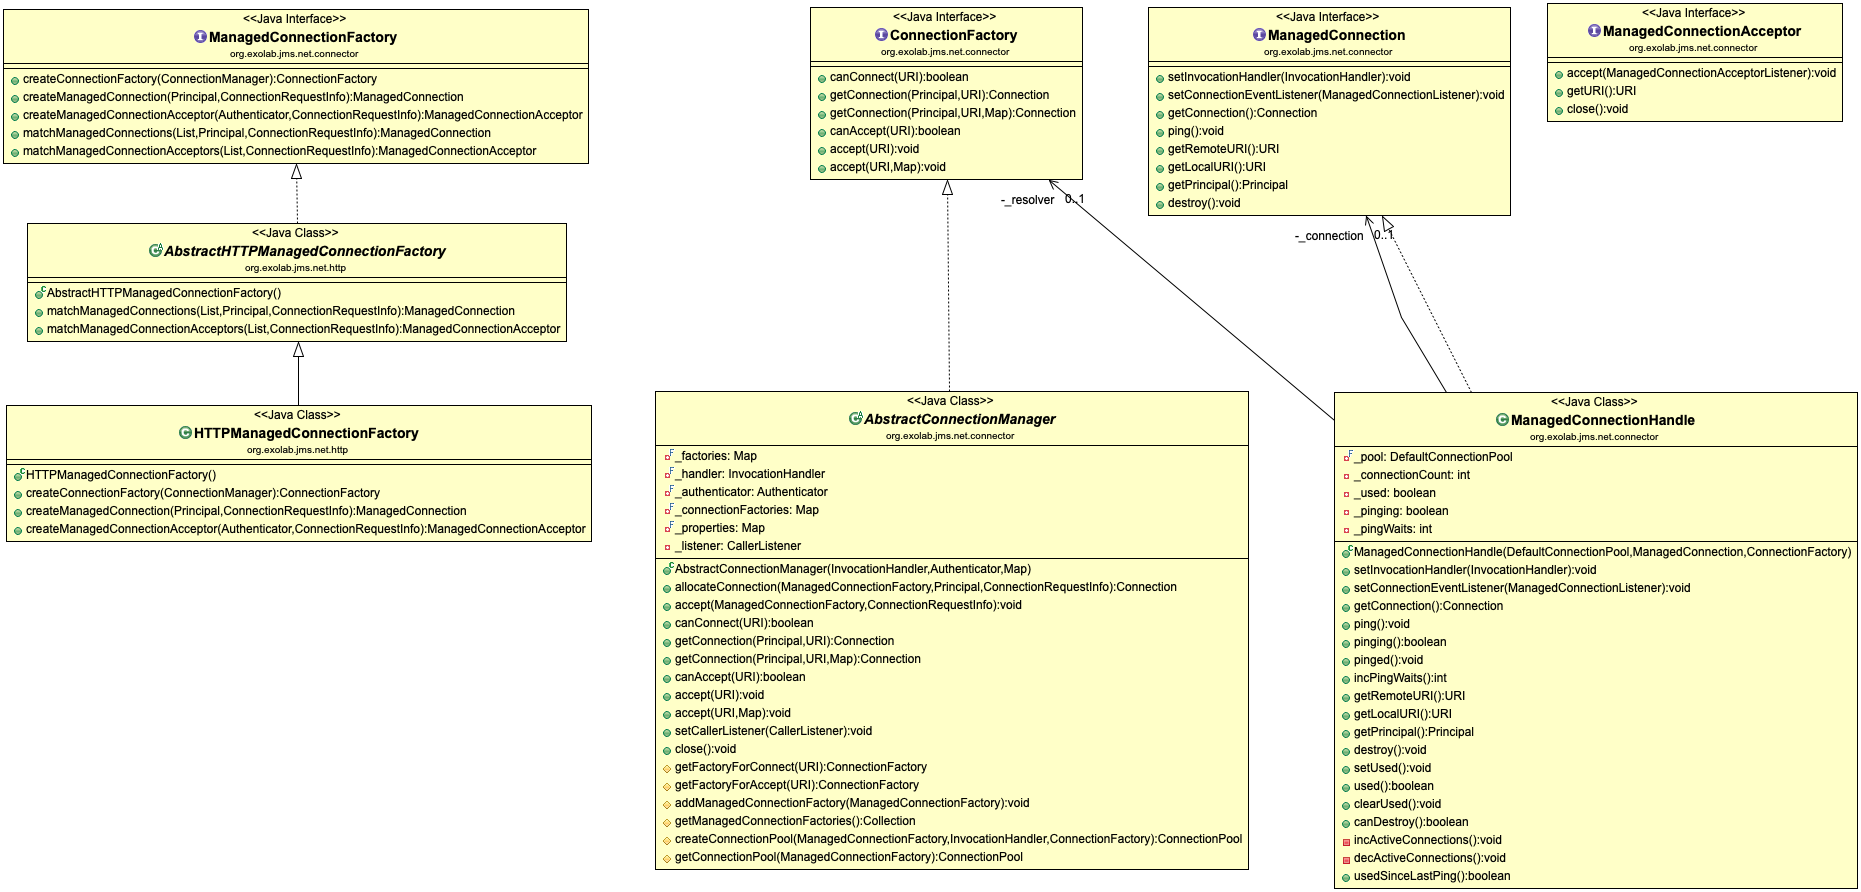
\includegraphics[width=\columnwidth]{images/abstract_factory.png}
    \caption{Abstract Factory design pattern in the project \textit{openjms}}
    \label{fig:abstract_factory}
\end{figure}
\FloatBarrier


An instance of the client class manages the connections. When it determines the connection that needs to be created, it passes the connection request info for the methods \texttt{createConnectionFactory}, \texttt{createManagedConnection}, \texttt{createManagedConnection\\Acceptor} of a \texttt{HTTPManagedConnectionFactory} object. The concrete class \texttt{HTTP\\ManagedConnectionFactory} extends the abstract class \texttt{AbstractHTTPManaged\\ConnectionFactory}. Additionally, the abstract class \texttt{AbstractHTTPManaged\\ConnectionFactory} implements the interface of the factory \texttt{ManagedConnection\\Factory}. The \texttt{Client} object can then use the \texttt{HTTPManagedConnectionFactory} object to create objects that create a new connection factory, a new connection, and an acceptor for connections. Figure~\ref{fig:managedConnectionFactory} presents the interface of the Abstract Factory pattern in the class \texttt{ManagedConnectionFactory}.

%--------------------------------------------------------------------------------------------%

\begin{figure}[htb]
\centering
\lstset{language=Java, basicstyle=\scriptsize, stepnumber=1, showspaces=false, showstringspaces=false,breaklines=true}
\begin{lstlisting}
public interface ManagedConnectionFactory {

    ConnectionFactory createConnectionFactory(ConnectionManager manager) 
        throws ResourceException;

    ManagedConnection createManagedConnection(Principal principal, 
         ConnectionRequestInfo info) throws ResourceException;

    ManagedConnectionAcceptor createManagedConnectionAcceptor(
        Authenticator authenticator, ConnectionRequestInfo info) 
        throws ResourceException;

    ManagedConnection matchManagedConnections(List connections, Principal principal,
        ConnectionRequestInfo info) throws ResourceException;

\end{lstlisting}
\caption{[Abstract Factory] ManagedConnectionFactory.java}
\label{fig:managedConnectionFactory}
\end{figure}
\FloatBarrier

%--------------------------------------------------------------------------------------------%

Figure~\ref{fig:AbstractHTTPManagedConnectionFactory} presents the abstract class that implements the interface \texttt{ManagedConnection\\Factory}.

\begin{figure}[htb]
\centering
\lstset{language=Java, basicstyle=\scriptsize,stepnumber=1, showspaces=false, showstringspaces=false,breaklines=true}
\begin{lstlisting}

public abstract class AbstractHTTPManagedConnectionFactory implements ManagedConnectionFactory {

    public ManagedConnection matchManagedConnections(List connections,
        Principal principal, ConnectionRequestInfo info) throws ResourceException {
        ManagedConnection result = null;

        if (info instanceof HTTPRequestInfo) {
            HTTPRequestInfo requestInfo = (HTTPRequestInfo) info;
            URI uri = URIHelper.convertHostToAddress(requestInfo.getURI());
            Iterator iterator = connections.iterator();
            while (iterator.hasNext()) {
                AbstractHTTPManagedConnection connection =
                        (AbstractHTTPManagedConnection) iterator.next();
                if (connection.hasPrincipal(principal)
                    && (uri.equals(connection.getRemoteURI())
                        || uri.equals(connection.getLocalURI()))) {
                    result = connection;
                    break;
                }
            }
        }
        return result;
    }

    public ManagedConnectionAcceptor matchManagedConnectionAcceptors(
            List acceptors, ConnectionRequestInfo info) throws ResourceException {
        ManagedConnectionAcceptor result = null;

        if (info instanceof SocketRequestInfo) {
            Iterator iterator = acceptors.iterator();
            while (iterator.hasNext()) {
                SocketManagedConnectionAcceptor acceptor =
                        (SocketManagedConnectionAcceptor) iterator.next();
                if (info.equals(acceptor.getRequestInfo())) {
                    result = acceptor;
                    break;
                }
            }
        }
        return result;
    }
}

\end{lstlisting}
\caption{[Abstract Factory] AbstractHTTPManagedConnectionFactory.java}
\label{fig:AbstractHTTPManagedConnectionFactory}
\end{figure}
\FloatBarrier

%--------------------------------------------------------------------------------------------%
Figure~\ref{fig:HTTPManagedConnectionFactory} presents the implementation of \texttt{HTTPManagedConnectionFactory}, the concrete class that extends \texttt{AbstractHTTPManagedConnectionFactory}. In this class, the method \texttt{createConnectionFactory} returns an object of the type \texttt{Connection\\Factory}, the method \texttt{createManagedConnection} returns an object of the type \texttt{HTTPManagedConnection}, and the method \texttt{createManagedConnectionAcceptor} returns an object of the type \texttt{ManagedConnectionAcceptor}. We present below the implementation of such classes. 

\begin{figure}[htb]
\centering
\lstset{language=Java, basicstyle=\scriptsize, stepnumber=1, showspaces=false, showstringspaces=false,breaklines=true}
\begin{lstlisting}


public class HTTPManagedConnectionFactory extends AbstractHTTPManagedConnectionFactory {

    public ConnectionFactory createConnectionFactory(ConnectionManager manager)
            throws ResourceException {
        return new HTTPConnectionFactory(this, manager);
    }

    public ManagedConnection createManagedConnection(Principal principal,
                                                     ConnectionRequestInfo info)
            throws ResourceException {
        if (!(info instanceof HTTPRequestInfo)) {
            throw new ResourceException("Argument 'info' must be of type "
                                        + HTTPRequestInfo.class.getName());
        }

        return new HTTPManagedConnection(principal, (HTTPRequestInfo) info);
    }

    public ManagedConnectionAcceptor createManagedConnectionAcceptor(
            Authenticator authenticator, ConnectionRequestInfo info)
            throws ResourceException {

        if (!(info instanceof SocketRequestInfo)) {
            throw new ResourceException("Argument 'info' must be of type "
                                        + SocketRequestInfo.class.getName());
        }

        return new HTTPManagedConnectionAcceptor(authenticator,
                                                 (SocketRequestInfo) info);
    }

}
\end{lstlisting}
\caption{[Abstract Factory] HTTPManagedConnectionFactory.java}
\label{fig:HTTPManagedConnectionFactory}
\end{figure}
\FloatBarrier

%--------------------------------------------------------------------------------------------%
Figure~\ref{fig:ConnectionFactory} presents the interface of \texttt{ConnectionFactory} and Figure~\ref{fig:AbstractConnectionManager} presents \texttt{Abstract\\ConnectionManager} that implements \texttt{ConnectionFactory}. This class is instantiated in the \texttt{HTTPManagedConnectionFactory} (see Figure~\ref{fig:HTTPManagedConnectionFactory}). It is responsible for managing connection factories, and their corresponding connection pools.

\begin{figure}[htb]
\centering
\lstset{language=Java, basicstyle=\scriptsize, stepnumber=1, showspaces=false, showstringspaces=false,breaklines=true}
\begin{lstlisting}
public interface ConnectionFactory {

    boolean canConnect(URI uri);

    Connection getConnection(Principal principal, URI uri) throws ResourceException;

    Connection getConnection(Principal principal, URI uri, Map properties) throws ResourceException;

    boolean canAccept(URI uri);

    void accept(URI uri) throws ResourceException;

    void accept(URI uri, Map properties) throws ResourceException;

}
\end{lstlisting}
\caption{[Abstract Factory] ConnectionFactory.java}
\label{fig:ConnectionFactory}
\end{figure}
\FloatBarrier

%--------------------------------------------------------------------------------------------%
\begin{figure}[htb]
\centering
\lstset{language=Java, basicstyle=\scriptsize, stepnumber=1, showspaces=false, showstringspaces=false,breaklines=true}
\begin{lstlisting}

public abstract class AbstractConnectionManager implements ConnectionManager, ConnectionFactory {

    // Attributes
       
    public AbstractConnectionManager(InvocationHandler handler, Authenticator authenticator, Map properties) {
        if (handler == null) { throw new IllegalArgumentException("Argument 'handler' is null");}
        if (authenticator == null) {
            throw new IllegalArgumentException(
                    "Argument 'authenticator' is null");
        }
        _handler = handler;
        _authenticator = authenticator;
        _properties = properties;
    }


    public void accept(ManagedConnectionFactory factory, ConnectionRequestInfo info) throws ResourceException {
        ConnectionPool pool = getConnectionPool(factory);
        ManagedConnectionAcceptor acceptor =
                pool.matchManagedConnectionAcceptors(info);
        if (acceptor == null) {
            acceptor = pool.createManagedConnectionAcceptor(_authenticator, info);
            acceptor.accept(pool.getManagedConnectionAcceptorListener());
        }
    }

    public boolean canConnect(URI uri) {
        ConnectionFactory factory = getFactoryForConnect(uri);
        return (factory != null);
    }

    public Connection getConnection(Principal principal, URI uri) throws ResourceException {
        return getConnection(principal, uri, null);
    }

    public Connection getConnection(Principal principal, URI uri, Map properties) throws ResourceException {
        ConnectionFactory factory = getFactoryForConnect(uri);
        if (factory == null) { throw new ResourceException("No connector for URI=" + uri);}
        return factory.getConnection(principal, uri, properties);
    }

    public boolean canAccept(URI uri) {
        ConnectionFactory factory = getFactoryForAccept(uri);
        return (factory != null);
    }

    public void accept(URI uri) throws ResourceException {
        accept(uri, null);
    }

    public void accept(URI uri, Map properties) throws ResourceException {
        ConnectionFactory factory = getFactoryForAccept(uri);
        if (factory == null) {throw new ResourceException("No connector for URI=" + uri);}
        factory.accept(uri, properties);
    }
    
    // Other methods
}

\end{lstlisting}
\caption{[Abstract Factory] AbstractConnectionManager.java}
\label{fig:AbstractConnectionManager}
\end{figure}
\FloatBarrier

%--------------------------------------------------------------------------------------------%
Figure~\ref{fig:ManagedConnection} presents the interface of \texttt{ManagedConnection} and Figure~\ref{fig:ManagedConnectionHandle} presents \texttt{Managed\\ConnectionHandle} that implements \texttt{ManagedConnection}. This class is instantiated in the \texttt{HTTPManagedConnectionFactory} (see Figure~\ref{fig:HTTPManagedConnectionFactory}). It is responsible for handling all connections.

\begin{figure}[htb]
\centering
\lstset{language=Java, basicstyle=\scriptsize, stepnumber=1, showspaces=false, showstringspaces=false,breaklines=true}
\begin{lstlisting}

public interface ManagedConnection {

    void setInvocationHandler(InvocationHandler handler) throws ResourceException;

    void setConnectionEventListener(ManagedConnectionListener listener) throws ResourceException;

    Connection getConnection() throws ResourceException;

    void ping() throws ResourceException;

    URI getRemoteURI() throws ResourceException;

    URI getLocalURI() throws ResourceException;

    Principal getPrincipal() throws ResourceException;

    void destroy() throws ResourceException;

}
\end{lstlisting}
\caption{[Abstract Factory] ManagedConnection.java}
\label{fig:ManagedConnection}
\end{figure}
\FloatBarrier

%--------------------------------------------------------------------------------------------%

\begin{figure}[htb]
\centering
\lstset{language=Java, basicstyle=\scriptsize, stepnumber=1, showspaces=false, showstringspaces=false,breaklines=true}
\begin{lstlisting}

final class ManagedConnectionHandle implements ManagedConnection {

    public void setInvocationHandler(InvocationHandler handler)
            throws ResourceException {
        _connection.setInvocationHandler(handler);
    }

     public void setConnectionEventListener(ManagedConnectionListener listener)
            throws ResourceException {
        _connection.setConnectionEventListener(listener);
    }

    public Connection getConnection() throws ResourceException {
        Connection connection = _connection.getConnection();
        return new ConnectionHandle(connection);
    }
    
    public synchronized void ping() throws ResourceException {
        try {
            _pinging = true;
            _pingWaits = 0;
            _connection.ping();
        } catch (ResourceException exception) {
            _pinging = false;
            throw exception;
        }
    }
    
    public URI getRemoteURI() throws ResourceException {
        return _connection.getRemoteURI();
    }
    
    public URI getLocalURI() throws ResourceException {
        return _connection.getLocalURI();
    }
    
    public Principal getPrincipal() throws ResourceException {
        return _connection.getPrincipal();
    }
    
    public void destroy() throws ResourceException {
        _connection.destroy();
    }
    
    // Other methods

}

\end{lstlisting}
\caption{[Abstract Factory] ManagedConnectionHandle.java}
\label{fig:ManagedConnectionHandle}
\end{figure}
\FloatBarrier

%--------------------------------------------------------------------------------------------%

Figure~\ref{fig:ManagedConnectionAcceptor} presents the interface of \texttt{ManagedConnectionAcceptor}. 
Although \texttt{Managed\\ConnectionAcceptor} is instantiated in \texttt{HTTPManagedConnectionFactory} (see Figure~\ref{fig:HTTPManagedConnectionFactory}), we could not find any class that implements this interface.

\begin{figure}[htb]
\centering
\lstset{language=Java, basicstyle=\scriptsize, stepnumber=1, showspaces=false, showstringspaces=false,breaklines=true}
\begin{lstlisting}

public interface ManagedConnectionAcceptor {

    void accept(ManagedConnectionAcceptorListener listener)
            throws ResourceException;

    URI getURI() throws ResourceException;
    
    void close() throws ResourceException;
}
\end{lstlisting}
\caption{[Abstract Factory] ManagedConnectionAcceptor.java}
\label{fig:ManagedConnectionAcceptor}
\end{figure}
\FloatBarrier
\section{Composite}

The composite pattern describes a group of objects that is treated the same way as a single instance of the same type of object. The intent of a composite is to ``compose" objects into tree structures to represent hierarchies. Implementing the composite pattern lets clients treat individual objects and compositions uniformly.

\subsection*{Example}

Figure~\ref{fig:composite} presents the composite design pattern found in the project \textit{lotus}. The interface \texttt{Decision} plays the role of \textit{Component}, the class \texttt{MultiDecision} plays the role of \textit{Composite}, and the classes \texttt{PassDecision} and \texttt{PlayLand} plays the role of \textit{leaf}.

\begin{figure}[htb]
    \centering
    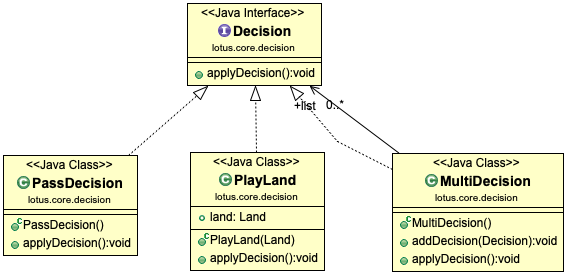
\includegraphics[width=0.8\columnwidth]{images/composite.png}
    \caption{Composite design pattern in the project \textit{lotus}}
    \label{fig:composite}
\end{figure}
\FloatBarrier

%--------------------------------------------------------------------------------------------%

An instance of the client manages the decision of the player. A decision is an action decided by the player. Figure~\ref{fig:Decision} presents the implementation of the interface \texttt{Decision} that contains only one method that applies the decision of the player.

\begin{figure}[!tbp]
\centering
\lstset{language=Java,  basicstyle=\scriptsize, stepnumber=1, showspaces=false, showstringspaces=false,breaklines=true}
\begin{lstlisting}

public interface Decision{
	public void applyDecision();
}

\end{lstlisting}
\caption{[Composite] Decision.java}
\label{fig:Decision}
\end{figure}
\FloatBarrier

%--------------------------------------------------------------------------------------------%
Figure~\ref{fig:MultiDecision} presents the implementation of the class \texttt{MultiDecision} that implements the interface \texttt{Decision}. This class represents multiple decisions as one decision.

\begin{figure}[!tbp]
\centering
\lstset{language=Java,  basicstyle=\scriptsize, stepnumber=1, showspaces=false, showstringspaces=false,breaklines=true}
\begin{lstlisting}
public class MultiDecision implements Decision {
	public ArrayList<Decision> list = new ArrayList<Decision>();
	
	public void addDecision(Decision d) {
		list.add(d);
	}
 
	public void applyDecision() {
		for(Decision d : list) {
			d.applyDecision();
		}
	}
}
\end{lstlisting}
\caption{[Composite] MultiDecision.java}
\label{fig:MultiDecision}
\end{figure}
\FloatBarrier

%--------------------------------------------------------------------------------------------%
Figure~\ref{fig: PlayLand} presents the implementation of the class \texttt{PlayLand} that also implements \texttt{Decision}. In this class, the player decided to play a land.

\begin{figure}[!tbp]
\centering
\lstset{language=Java,  basicstyle=\scriptsize, stepnumber=1, showspaces=false, showstringspaces=false,breaklines=true}
\begin{lstlisting}

public class PlayLand implements Decision {
	public Land land;
	public PlayLand(Land l) {
		land = l;
	}
	public void applyDecision() {
		ChangeZone eff = new ChangeZone(land,land.zone,land.owner.inPlay);
		eff.resolve();
	}
}
\end{lstlisting}
\caption{[Composite] PlayLand.java}
\label{fig: PlayLand}
\end{figure}
\FloatBarrier

%--------------------------------------------------------------------------------------------%
Figure~\ref{fig:PassDecision} presents the implementation of the class \texttt{PassDecision} that also implements \texttt{Decision}. In this class, the played decided do anything, i.e., pass the decision.

\begin{figure}[!tbp]
\centering
\lstset{language=Java,  basicstyle=\scriptsize, stepnumber=1, showspaces=false, showstringspaces=false,breaklines=true}
\begin{lstlisting}

public class PassDecision implements Decision {
	public void applyDecision() {
		// Decision to pass, ie do nothing
	}
}

\end{lstlisting}
\caption{[Composite] PassDecision.java}
\label{fig:PassDecision}
\end{figure}
\FloatBarrier

%--------------------------------------------------------------------------------------------%
\section{Iterator}

This iterator pattern is a pattern used to get access to the elements of a collection in a object secuentially without the need to know or expose its underlying representation.

% Description of the design pattern

\subsection*{Role}

The Iterator pattern here plays the role to secure the elements of the collections. SimplePrincipalCollection play the role of the internal design of the iterator, while the DelegatingSubject is the security layer that handles the collection and the other interfaces that extend the collections withouth exposing all elements of the collection.

\subsection*{Example}

\begin{center}
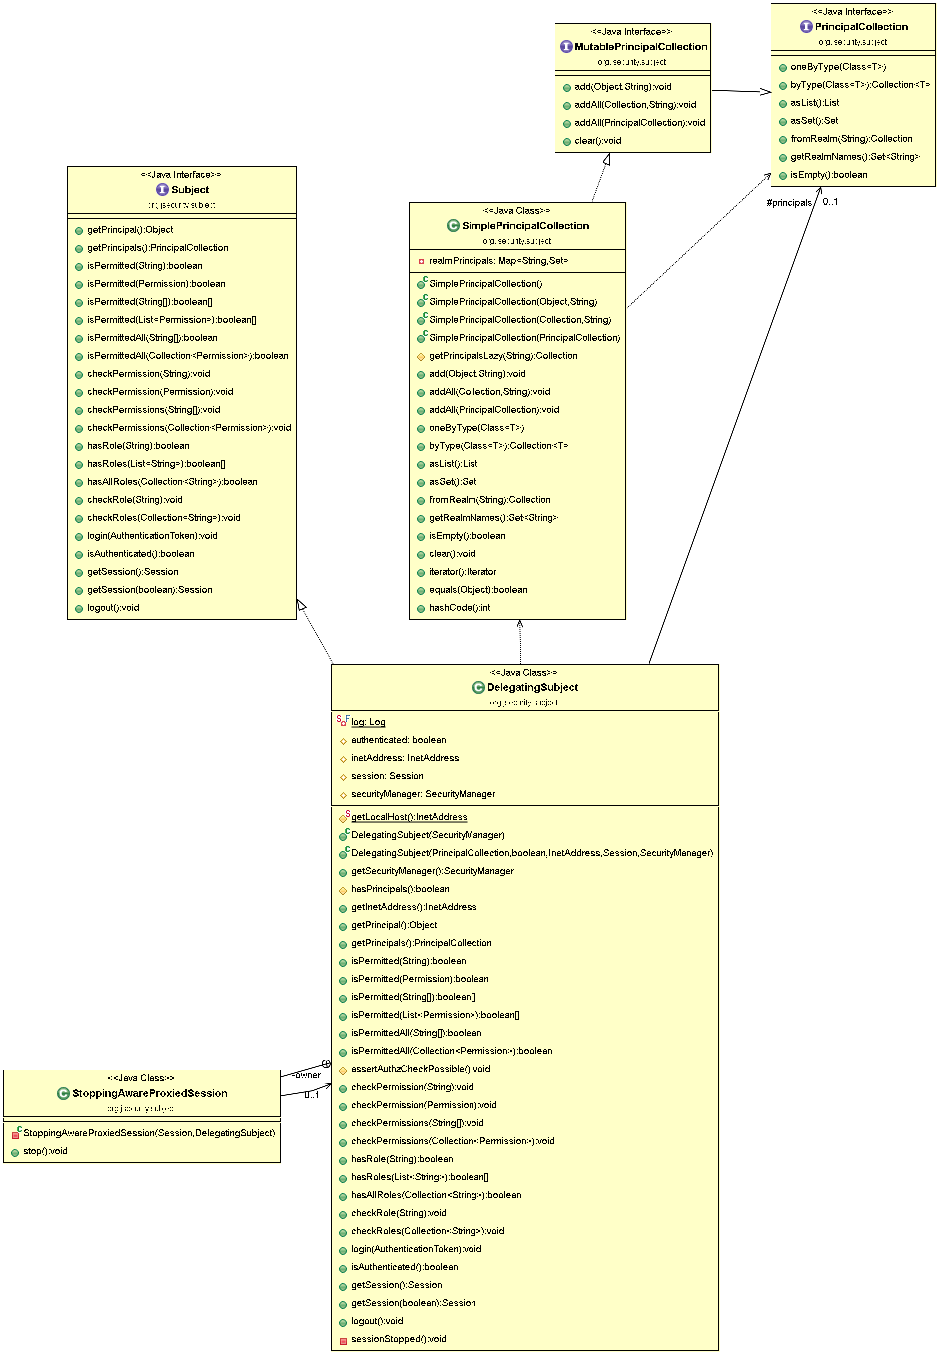
\includegraphics[width=16cm, height=19cm]{images/iterator.png}
\end{center}

In the program "18_jsecurity" in "org.jsecurity.subject/SimplePrincipalCollection" class that implements the MutablePrincipalCollection in which they implement an internal design of the iterator for the collection:

\begin{figure}[!tbp]
\centering
\lstset{language=Java, stepnumber=1, showspaces=false, showstringspaces=false,breaklines=true}
\begin{lstlisting}

public class SimplePrincipalCollection implements MutablePrincipalCollection {

    private Map<String, Set> realmPrincipals;

    public SimplePrincipalCollection() {
    }

    public SimplePrincipalCollection(Object principal, String realmName) {
        if (principal instanceof Collection) {
            addAll((Collection) principal, realmName);
        } else {
            add(principal, realmName);
        }
    }

    public SimplePrincipalCollection(Collection principals, String realmName) {
        addAll(principals, realmName);
    }

    public SimplePrincipalCollection(PrincipalCollection principals) {
        addAll(principals);
    }

    protected Collection getPrincipalsLazy(String realmName) {
        if (realmPrincipals == null) {
            realmPrincipals = new LinkedHashMap<String, Set>();
        }
        Set principals = realmPrincipals.get(realmName);
        if (principals == null) {
            principals = new LinkedHashSet();
            realmPrincipals.put(realmName, principals);
        }
        return principals;
    }

    public void add(Object principal, String realmName) {
        if (realmName == null) {
            throw new IllegalArgumentException("realmName argument cannot be null.");
        }
        if (principal == null) {
            throw new IllegalArgumentException("principal argument cannot be null.");
        }
        getPrincipalsLazy(realmName).add(principal);
    }

    public void addAll(Collection principals, String realmName) {
        if (realmName == null) {
            throw new IllegalArgumentException("realmName argument cannot be null.");
        }
        if (principals == null) {
            throw new IllegalArgumentException("principals argument cannot be null.");
        }
        if (principals.isEmpty()) {
            throw new IllegalArgumentException("principals argument cannot be an empty collection.");
        }
        getPrincipalsLazy(realmName).addAll(principals);
    }

    public void addAll(PrincipalCollection principals) {
        if (principals.getRealmNames() != null) {
            for (String realmName : principals.getRealmNames()) {
                for (Object principal : principals.fromRealm(realmName)) {
                    add(principal, realmName);
                }
            }
        }
    }

    public <T> T oneByType(Class<T> type) {
        if (realmPrincipals == null || realmPrincipals.isEmpty()) {
            return null;
        }
        Collection<Set> values = realmPrincipals.values();
        for (Set set : values) {
            for (Object o : set) {
                if (type.isAssignableFrom(o.getClass())) {
                    return (T) o;
                }
            }
        }
        return null;
    }

    public <T> Collection<T> byType(Class<T> type) {
        if (realmPrincipals == null || realmPrincipals.isEmpty()) {
            return Collections.EMPTY_SET;
        }
        Set<T> typed = new LinkedHashSet<T>();
        Collection<Set> values = realmPrincipals.values();
        for (Set set : values) {
            for (Object o : set) {
                if (type.isAssignableFrom(o.getClass())) {
                    typed.add((T) o);
                }
            }
        }
        if (typed.isEmpty()) {
            return Collections.EMPTY_SET;
        }
        return Collections.unmodifiableSet(typed);
    }

    public List asList() {
        Set all = asSet();
        if (all.isEmpty()) {
            return Collections.EMPTY_LIST;
        }
        return Collections.unmodifiableList(new ArrayList(all));
    }

    public Set asSet() {
        if (realmPrincipals == null || realmPrincipals.isEmpty()) {
            return Collections.EMPTY_SET;
        }
        Set aggregated = new LinkedHashSet();
        Collection<Set> values = realmPrincipals.values();


    public Iterator iterator() {
        return asSet().iterator();
    }
\end{lstlisting}
\caption{SimplePrincipalColletion.java}
\label{SimplePrincipalColletion}
\end{figure}

In the interface in MutablePrincipalCollection, we can see it extends the principal collection adding all the principals to the given collection.

\begin{figure}[!tbp]
\centering
\lstset{language=Java, stepnumber=1, showspaces=false, showstringspaces=false,breaklines=true}
\begin{lstlisting}

public interface MutablePrincipalCollection extends PrincipalCollection {

    void add(Object principal, String realmName);

     void addAll(Collection principals, String realmName);

    void addAll(PrincipalCollection principals);


    void clear();
}
\end{lstlisting}
\caption{AttributeModelBuilder.java}
\label{AttributeModelBuilder}
\end{figure}

In the interface PrincipalCollection they return the collection info necessary in different functions:

\begin{figure}[!tbp]
\centering
\lstset{language=Java, stepnumber=1, showspaces=false, showstringspaces=false,breaklines=true}
\begin{lstlisting}

public interface PrincipalCollection extends Iterable, Serializable {

    <T> T oneByType(Class<T> type);
    <T> Collection<T> byType(Class<T> type);
    List asList();
    Set asSet();
    Collection fromRealm(String realmName);
    Set<String> getRealmNames();
    boolean isEmpty();
}

\end{lstlisting}
\caption{PrincipalCollection.java}
\label{PrincipalCollection}
\end{figure}

The DelegatingSubject class, delegates the method calls and iterates the objects withouth exposing the whole colection:

\begin{figure}[!tbp]
\centering
\lstset{language=Java, stepnumber=1, showspaces=false, showstringspaces=false,breaklines=true}
\begin{lstlisting}

    public DelegatingSubject(PrincipalCollection principals, boolean authenticated, InetAddress inetAddress,
                             Session session, SecurityManager securityManager) {
        if (securityManager == null) {
            throw new IllegalArgumentException("SecurityManager argument cannot be null.");
        }
        this.securityManager = securityManager;
        this.principals = principals;

        this.authenticated = authenticated;

        if (inetAddress != null) {
            this.inetAddress = inetAddress;
        } else {
            this.inetAddress = getLocalHost();
        }
        if (session != null) {
            this.session = new StoppingAwareProxiedSession(session, this);
        }
    }
    public Object getPrincipal() {
        PrincipalCollection principals = getPrincipals();
        if (principals == null || principals.isEmpty()) {
            return null;
        }
        return principals.asSet().iterator().next();
    }

    public PrincipalCollection getPrincipals() {
        return this.principals;
    }

\end{lstlisting}
\caption{DelegatingSubject.java}
\label{DelegatingSubject}
\end{figure}

The Subject interface just gets the Objects and Principal Collection and check the role of each element:

\begin{figure}[!tbp]
\centering
\lstset{language=Java, stepnumber=1, showspaces=false, showstringspaces=false,breaklines=true}
\begin{lstlisting}
public interface Subject {

    Object getPrincipal();
    PrincipalCollection getPrincipals();
    boolean hasAllRoles(Collection<String> roleIdentifiers);
    void checkRole(String roleIdentifier) throws AuthorizationException;
    void checkRoles(Collection<String> roleIdentifiers) throws AuthorizationException;

...
}
\end{lstlisting}
\caption{Subject.java}
\label{Subject}
\end{figure}

\section{Observer}

The observer pattern is a software design pattern in which an object, called the subject, maintains a list of its dependents, called observers, and notifies them automatically of any state changes, usually by calling one of their methods. The observer pattern can cause memory leaks, known as the lapsed listener problem, because in basic implementation it requires both explicit registration and explicit deregistration, as in the dispose pattern, because the subject holds strong references to the observers, keeping them alive. This can be prevented by the subject holding weak references to the observers.

% Description of the design pattern
\subsection*{Example}

Figure~\ref{fig:Observer} presents the UML diagram of observer design pattern of project \textit{Follow}. In this diagram the \texttt{OutputDestination} interface is playing the role of observer and the class \texttt{FileFollowers} class is playing the role of subject for the observer design pattern.      

\begin{figure}[htb]
    \centering
    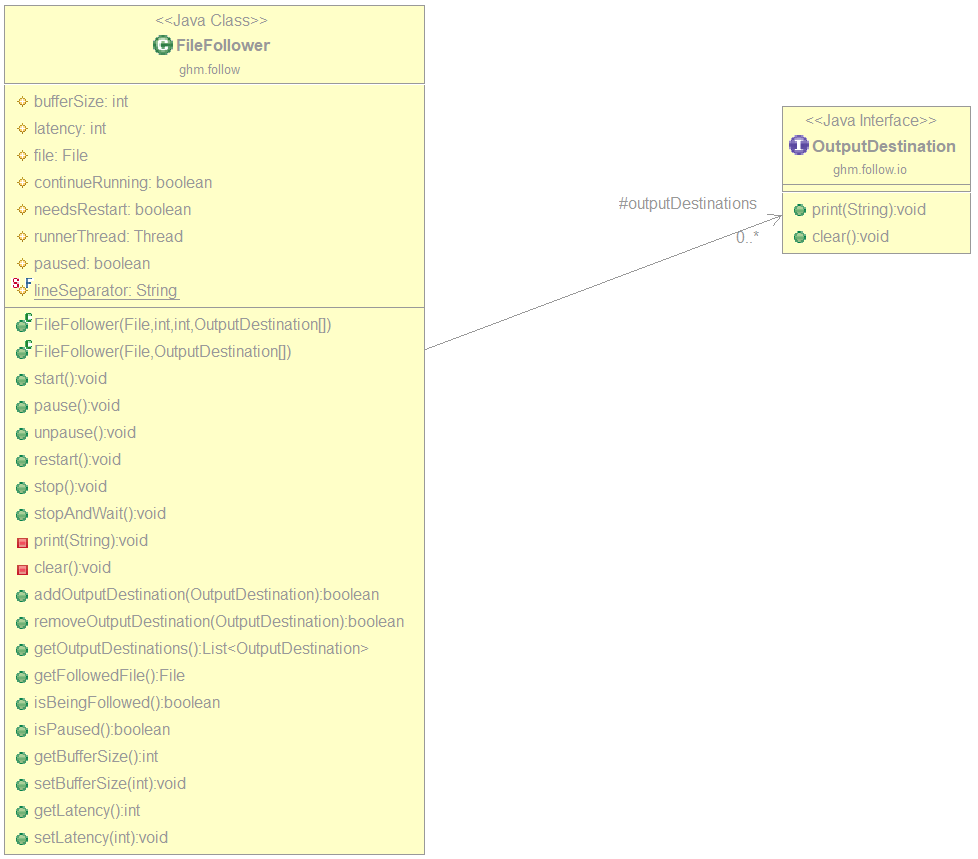
\includegraphics[width=\columnwidth]{images/Observer.png}
    \caption{Observer design pattern in the project \textit{Follow}}
    \label{fig:Observer}
\end{figure}
\FloatBarrier

% Description of the roles of the class in the design pattern

In Figure~\ref{fig:OutputDestination} observer interface has two methods \texttt{print} and \texttt{clear} and as you can see in the Figure~\ref{fig:FileFollower} and Figure~\ref{fig:Observer} the subject (i.e. \texttt{FileFollower}) has two common method with the observer that they can notify Observer about any changes, so that means \texttt{FileFollower} as subject for observer design pattern would not update itself directly and just call a method from \texttt{OutputDestination} interface as observer design pattern. 

%----------------------------------------------------------------------------------%
\begin{figure}[htb]
\centering
\lstset{language=Java, basicstyle=\scriptsize, stepnumber=1, showspaces=false, showstringspaces=false,breaklines=true}
\begin{lstlisting}

public class FileFollower {

	public FileFollower(File file, int bufferSize, int latency,
	        OutputDestination[] initialOutputDestinations) {
		this.file = file;
		this.bufferSize = bufferSize;
		this.latency = latency;

		int initOutputDestsSize = (initialOutputDestinations != null) ? initialOutputDestinations.length
		        : 0;
		outputDestinations = new ArrayList<OutputDestination>(initOutputDestsSize);
		for (int i = 0; i < initOutputDestsSize; i++) {
			outputDestinations.add(initialOutputDestinations[i]);
		}
	}


	public FileFollower(File file, OutputDestination[] initialOutputDestinations) {
		        initialOutputDestinations);
	}


	public synchronized void start() {
		if (continueRunning && paused) {
			unpause();
		}
		else {
			continueRunning = true;
			paused = false;
			runnerThread = new Thread(new Runner(), getFollowedFile().getName());
			runnerThread.start();
		}
	}

	public synchronized void pause() {
		paused = true;
	}

	public synchronized void unpause() {
		paused = false;
	}

	public synchronized void restart() {
		needsRestart = true;
		runnerThread.interrupt();
	} //Other method

\end{lstlisting}
\caption{[Observer] FileFollower.java}
\label{fig:FileFollower}
\end{figure}
\FloatBarrier

%------------------------------------------------------------------------------------%
\begin{figure}[htb]
\centering
\lstset{language=Java, basicstyle=\scriptsize, stepnumber=1, showspaces=false, showstringspaces=false,breaklines=true}
\begin{lstlisting}
public interface OutputDestination {
	public void print(String s);
	public void clear();
}
\end{lstlisting}
\caption{[Observer] OutputDestination.java}
\label{fig:OutputDestination}
\end{figure}
\FloatBarrier
%------------------------------------------------------------------------------------%




\section{Singleton}

The singleton pattern is a software design pattern that restricts the instantiation of a class to one object. This is useful when exactly one object is needed to coordinate actions across the system.

\subsection*{Role}
The pattern involves a single class which create and object like while making sure that only single object is created.

\subsection*{Example}

The following Singleton pattern was found in the following instance: 'w.tools.explorer.model.Attri-
buteModelBuilder::singleton:fw.tools.explorer.model.AttributeModelBuilder'

\begin{center}
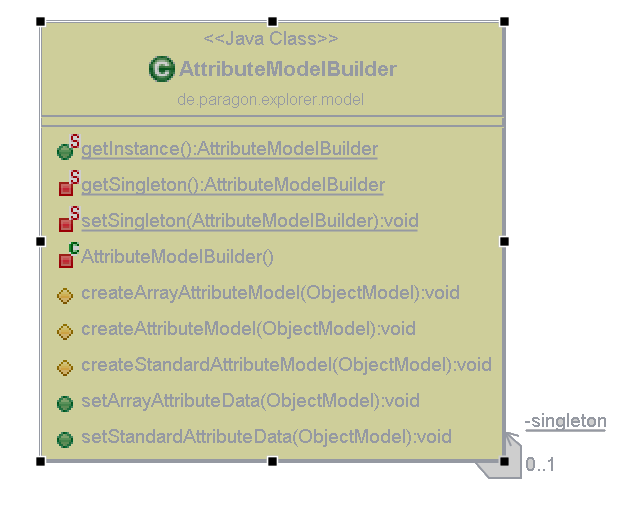
\includegraphics{images/Singleton.png}
\end{center}


In the function AttributeModelBuilder we can see the instance receiving the instance of an Object and we can see how it obtains a single object:

% \begin{spverbatim}
% public final class AttributeModelBuilder {
% 	private static AttributeModelBuilder	singleton;

% 	public static AttributeModelBuilder getInstance() {
% 		return AttributeModelBuilder.getSingleton();
% 	}
% 	private static AttributeModelBuilder getSingleton() {
% 		if (AttributeModelBuilder.singleton == null) {
% 			AttributeModelBuilder.setSingleton(new AttributeModelBuilder());
% 		}
% 		return AttributeModelBuilder.singleton;
% 	}
% 		private static void setSingleton(AttributeModelBuilder builder) {
% 		AttributeModelBuilder.singleton = builder;
% 	}
% ....}
% \end{spverbatim}


\begin{figure}[!tbp]
\centering
\lstset{language=Java, stepnumber=1, showspaces=false, showstringspaces=false,breaklines=true}
\begin{lstlisting}
 static {
         public final class AttributeModelBuilder {
	private static AttributeModelBuilder	singleton;

	public static AttributeModelBuilder getInstance() {
		return AttributeModelBuilder.getSingleton();
	}
	private static AttributeModelBuilder getSingleton() {
		if (AttributeModelBuilder.singleton == null) {
			AttributeModelBuilder.setSingleton(new AttributeModelBuilder());
		}
		return AttributeModelBuilder.singleton;
	}
		private static void setSingleton(AttributeModelBuilder builder) {
		AttributeModelBuilder.singleton = builder;
	}
}
                }
             }
          );
 }
\end{lstlisting}
\caption{AttributeModelBuilder.java}
\label{AttributeModelBuilder}
\end{figure}
\section{Visitor}

\subsection{Definition}

\subsection{Role}

\subsection{Example}


\end{document}
